\chapter{Framework evaluation}

In this chapter we will look at an evaluation framework developed at the institute for program structures and data organization. We will go over its goal, a basic overview of its components and how it is meant to be used. Finally we will talk about the challenges of implementing an analysis using shap withing this framework.

\section{Goal of the framework}

As discussed in \autoref{ch:Introduction}, tools are essential for the mass adoption of new technologies. XAI is still met with a lot of scepticism and rightfully so, every new technology should be tested extensively before it is widely adopted. Our evaluations took over a year to produce and we believe that by using the same framework we developed other scientists can create further evaluations in much less time.

\section{Overview of the framework}

\textit{The following description of our framework is a simplification, please refer to the documentation or actual code for a truthful representation. This is especially true for the overview diagram \autoref{fig:framework_overview}. This was done for overview purposes.}


The framework can be divided into 5 distinct parts which in theory should be exchangeable without having to modify any of the other 4 parts.

\begin{enumerate}
    \item Resources, \textit{data set, embedding, preprocessing}
    \item Classifiers, \textit{abstract classifier class, fit function, classification function}
    \item Explainers, \textit{abstract explainer class, explain function}
    \item Analyses
    \item Output, \textit{functions to save the analysis data in csv files for further processing.}
\end{enumerate}

In \autoref{fig:framework_overview} I provide the overview over the five components and their interfaces.

\begin{figure}[H]
    \centering
    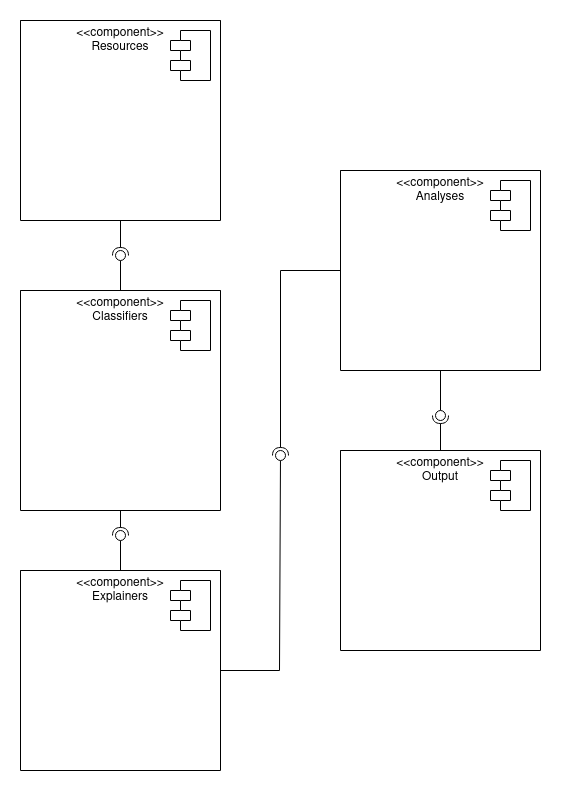
\includegraphics[width=\linewidth]{images/05_framework_eval/Component_diagram_overview_framework.png}
    \caption{Component diagram, framework overview}
    \label{fig:framework_overview}
\end{figure}

\subsection{Component 1: Resources}

\begin{figure}[H]
    \centering
    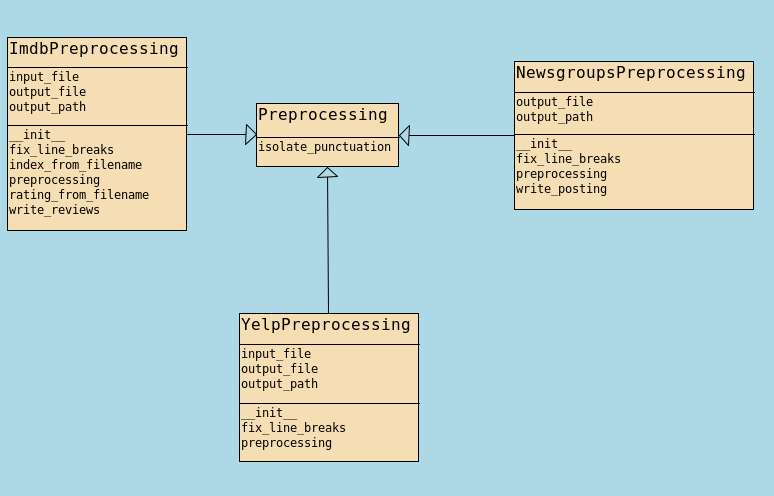
\includegraphics[width=\linewidth]{images/05_framework_eval/Preprocessing.png}
    \caption{Preprocessing}
    \label{fig:preprocessing}
\end{figure}

The \textit{Resource} component includes the data set and any preprocessing functions which might be needed to prepare/modify the given dataset. If you decide to use/include your own dataset, and you need to preprocess your data, you should make a child class to the preprocessing class.

\subsection{Component 2: Classifiers}

\begin{figure}[H]
    \centering
    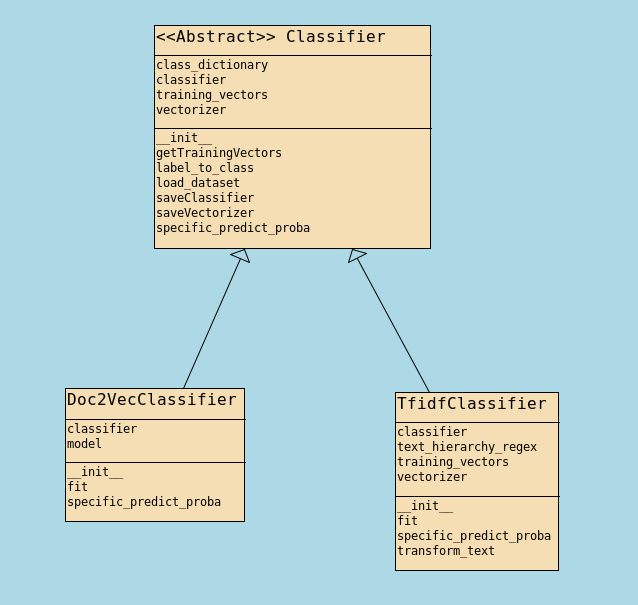
\includegraphics[width=\linewidth]{images/05_framework_eval/Classifiers.png}
    \caption{Classifiers}
    \label{fig:Classifiers}
\end{figure}

The \textit{Classification} component includes the classifiers, with functions to train or load them. Pretrained classifiers are not supported yet, but you can save a classifier after training it. A new classifier should be a child to the abstract classifier class.

\subsection{Component 3: Explainers}

\begin{figure}[H]
    \centering
    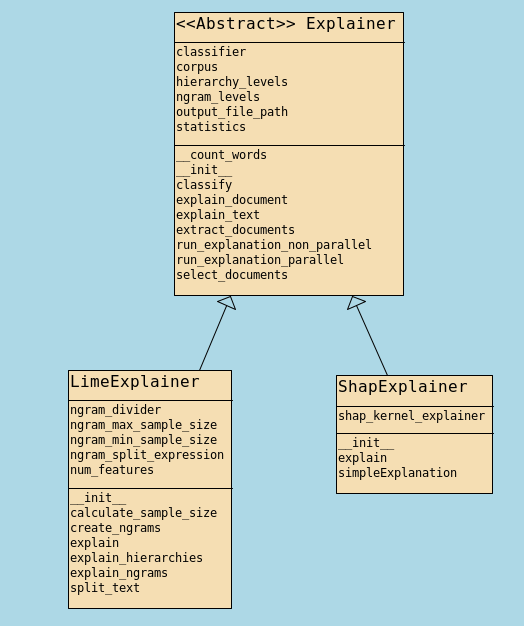
\includegraphics[width=\linewidth]{images/05_framework_eval/Explainers.png}
    \caption{Explainers}
    \label{fig:Explainers}
\end{figure}

The \textit{Explainer} component includes the explainers and functions to explain texts or documents.
If you wish to add another explainer, it should be a child class of the abstract explainer class. This can be challenging, because the output format of the explanation must follow a certain format.

\subsection{Component 4: Analyses}


\begin{figure}[H]
    \centering
    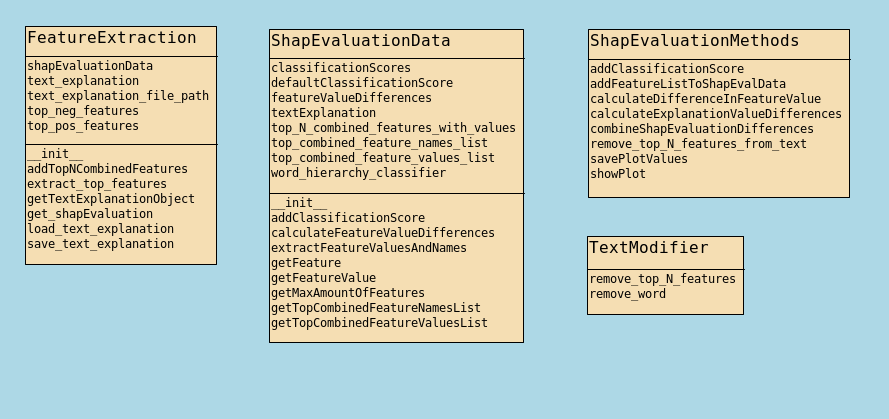
\includegraphics[width=\linewidth]{images/05_framework_eval/Analyses.png}
    \caption{Analyses}
    \label{fig:Analyses}
\end{figure}

The \textit{Analyses} component is much more loosely structured. The user should be able to freely carry out his own analyses.

\subsection{Component 5: Output}

\begin{figure}[H]
    \centering
    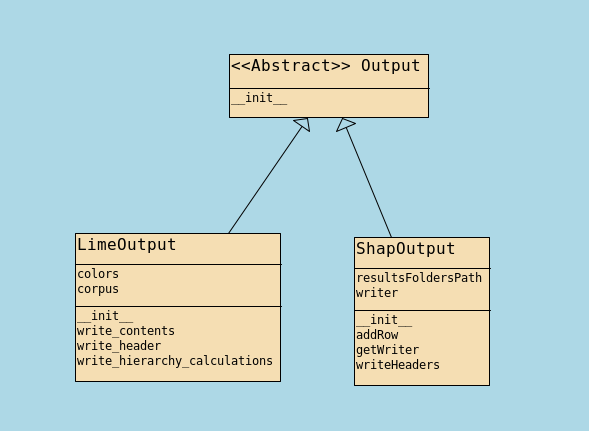
\includegraphics[width=\linewidth]{images/05_framework_eval/Output.png}
    \caption{Output}
    \label{fig:Output}
\end{figure}

The \textit{Output} component defines how the analysis data is saved. Here we break the modularity of the framework. If you add another analysis, it is very likely, that you will have to write your own output child class. We are working on improving this, hopefully this will not be necessary in the future.

\section{Intended use}

We do not expect you to be satisfied with the provided components, depending on the scope of your work, you might want to exchange multiple components. Nonetheless, you might still find our framework useful. A major difficulty in setting up an XAI analysis, is that it can take months of coding to get an analysis to work properly. We suggest you build it step by step, working on one component at a time and using our provided ones to check for mistakes and provide structure to your workflow.

\section{Shap Implementation using our framework}

There are many different implementations of the shap algorithm, notably \textit{gradientexplainer, deepexplainer, linearexplainer} and \textit{kernelexplainer}. Except for \textit{kernelexplainer}, each one is specialized for a special type of neural network. Since our framework is intended to have modular, interchangeable components, I tried to use \textit{kernelexplainer} in our analysis.

During development, I encountered following challenges:
\begin{itemize}
    \item Kernelshap's poor performance
    \item Kernelshap's resource requirements
    \item Missing required function in the library
\end{itemize}

Let's go over them in detail:
\subsection{Poor performance}

Kernelshap is model agnostic (meaning it can work with every type of artificial neural network) which meant that it could not be optimized according to the shape of the respective neural network. Because of that, generating an explanation for a single text took between 5 to 10 minutes on my workstation and the institutes server alike. This is very hindersome during development. While impossible to completely solve, I took some measures to cache as many steps as possible.

\begin{lstlisting}
    def saveClassifier(self, classifier_out_file):
        print("saving classifier: ", classifier_out_file)
        dump(self.classifier, classifier_out_file)

    def saveVectorizer(self, vectorizer_out_file):
        print("saving vectorizer:", vectorizer_out_file)
        dump(self.vectorizer, vectorizer_out_file)
\end{lstlisting}

\subsection{Resource requirements}

Kernelshap uses a lot of memory. You need around 10 GB of ram to run an explanation for a single text. Since this is hard-coded into the shap library, not many optimizations were possible. I upgraded my hardware and added parameters to limit the amount of texts being explained in parallel.

\begin{lstlisting}
    if RUNNING_ON_SERVER:
        # how many cpus are used during parallelization. With more than 2 my pc crashes
        AMOUNT_OF_CPU_CORES = 10
    else
        # how many cpus are used during parallelization. With more than 2 my pc crashes
        AMOUNT_OF_CPU_CORES = 2
\end{lstlisting}

\begin{lstlisting}
    pool = mp.Pool(shap_constants.AMOUNT_OF_CPU_CORES)
    # the actual explanation is now saved inside of this array of textExplanations
    text_explanations = pool.starmap(self.explain_document, explain_documents_arguments_iterable_tuple)

    pool.close()
\end{lstlisting}

\subsection{Missing functions in library}

Shap is a young explainer in active development. A few API functions which were necessary for my analysis weren't provided, so I had to write them myself. One example is that it was not possible to get a list of the top N features which have the most impact on the classification score. It was especially challenging to write this function, since the documentation on how to extract these values is nonexistent. It was thus necessary, to analyse the library's code line by line.

\begin{lstlisting}
def get_top_features_of_specific_class(index: int, amount_of_features: int, shap_values, feature_names, pos_or_neg_val: str):
    '''
    :param index: 0 for first class, 1 for second class, doesn't matter since the pos ones for one class are the neg
    ones for the other but we encourage to only use class 1 to avoid confusion.
    :param amount_of_features: how many features should be presented in the explanation
    :param shap_values: I believe those to be of the same format as the model output: in our case the model outputs
    2 values so the shap_values are a list with two arrays. first array: shapley_values[0] holds the features which are
    believed to nudge the explanation towards class 0,     shapley_values[1] hold the values which are believed to
    nudge the explanation towards class 1.
    :param feature_names: the model takes text transformed in vector form, the explanation should output text again.
    feature names map the vector values back to text.
    :return: top <amount_of_features> for class <class_number> as a table.
    '''
    # extract top features either positive or negative
    if pos_or_neg_val == "pos":
        shap_class_values = shap_values[index].mean(axis=0)
    elif pos_or_neg_val == "neg":
        shap_class_values = - shap_values[index].mean(axis=0)
    elif pos_or_neg_val == "combined":
        shap_class_values = np.abs(shap_values[index]).mean(axis=0)

    importance_df = pd.DataFrame([feature_names, shap_class_values.tolist()]).T
    importance_df.columns = ['feature-name', 'shap_importance']
    importance_df = importance_df.sort_values('shap_importance', ascending=False)
    return importance_df.head(amount_of_features)
\end{lstlisting}

%\subsection{Adapting for text-input}

\section{Framework outlook}

The Framework is still a work in progress. Most notably it lacks documentation and overview to reduce the entry barrier. That being said, once its architecture adheres to \autoref{fig:framework_overview} and some basic documentation is provided, I believe that it has the potential to contribute in a significant way to future XAI analyses.